\documentclass[12pt]{article}
\usepackage{graphicx}
\usepackage{geometry}
\geometry{a4paper, margin=1in}

\begin{document}

\begin{center}
\includegraphics[width=3cm]{images/logo.jpg}
\end{center}

\begin{center}
\Large{\textbf{ARM 2010 EC Question 39}}
\end{center}

\vspace{0.5cm}

\noindent
\textbf{Name:} Harshita N Kumar \\
\textbf{ID:} COMETFWC052

\vspace{0.5cm}

\section*{Question}

39) The Boolean function realized by the logic circuit shown is

\vspace{0.5cm}

\begin{tabular}{ll}
a) $F = \Sigma m(0,1,3,5,9,10,14)$ & c) $F = \Sigma m(1,2,4,5,11,14,15)$ \\[0.4cm]
b) $F = \Sigma m(2,3,5,7,8,12,13)$ & d) $F = \Sigma m(2,3,5,7,8,9,12)$
\end{tabular}

\vspace{0.7cm}

\section*{Question Analysis}

The Boolean function is expressed using the summation of minterms notation. The notation $\Sigma m$ indicates that the function output becomes 1 for the specified minterm indices and 0 for all other input combinations.

Since the highest minterm value is 15, the function consists of four variables. A four-variable Boolean function generates $2^4 = 16$ possible input combinations ranging from decimal 0 to decimal 15.

By observing the implemented circuit and experimental results, the output becomes 1 for the input combinations:

$0,1,3,5,9,10,14$

Thus, the correct option is:

$a) F = \Sigma m(0,1,3,5,9,10,14)$

All other options produce different output combinations and therefore do not match the circuit behavior.

\section*{Truth Table}

\begin{center}
\begin{tabular}{|c|c|}
\hline
Input & F \\
\hline
0  & 1 \\
1  & 1 \\
2  & 0 \\
3  & 1 \\
4  & 0 \\
5  & 1 \\
6  & 0 \\
7  & 0 \\
8  & 0 \\
9  & 1 \\
10 & 1 \\
11 & 0 \\
12 & 0 \\
13 & 0 \\
14 & 1 \\
15 & 0 \\
\hline
\end{tabular}
\end{center}

The truth table confirms that the function output is 1 only for the specified minterms and 0 otherwise.

\section*{Hardware Implementation}

The Boolean function was implemented using Raspberry Pi Pico 2W. The microcontroller generates input values from 0 to 15 using a loop. For each value, the program checks whether the input belongs to the minterm set.

If the input is present in the set, the output becomes 1. Otherwise, the output becomes 0.

The seven-segment display shows the output value, and an LED is used as an additional visual indicator. When $F = 1$, the LED turns ON and the display shows 1. When $F = 0$, the LED turns OFF and the display shows 0.

\begin{center}
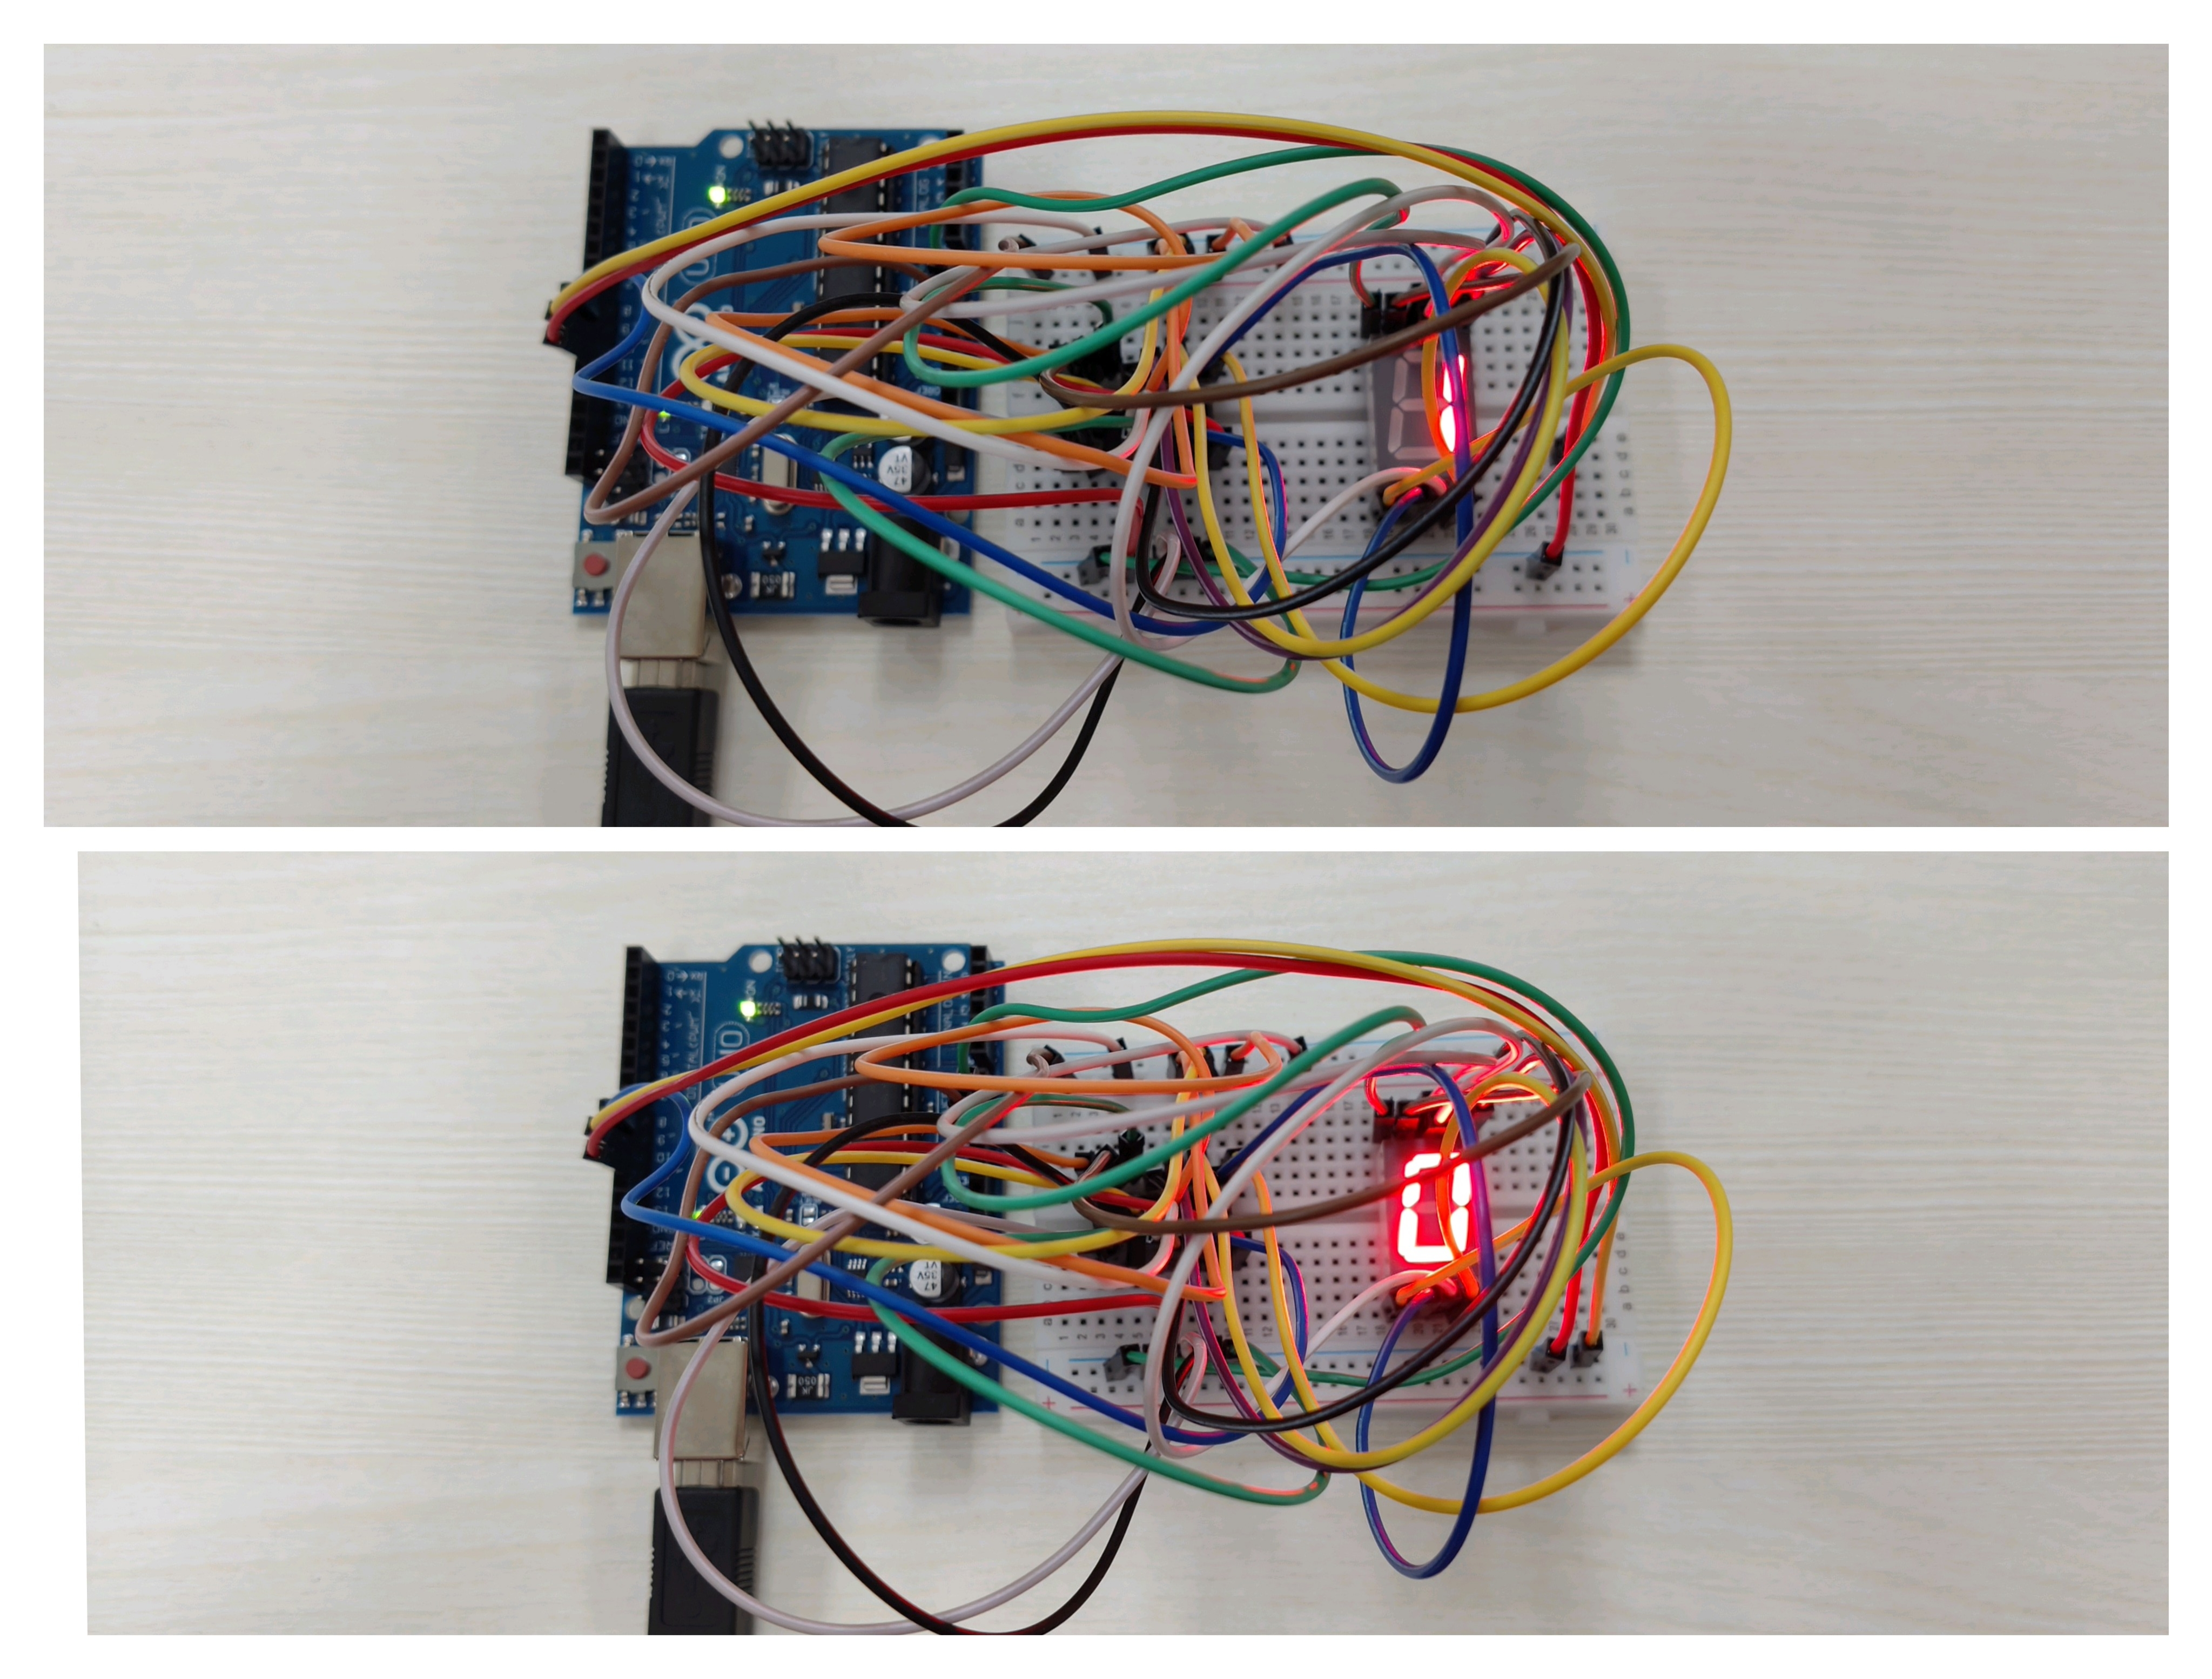
\includegraphics[width=9cm]{images/hardware.jpg}
\end{center}

\section*{Required Components and Pin Connections}

Components used in the experiment:

\begin{itemize}
\item Raspberry Pi Pico 2W
\item Seven Segment Display
\item LED
\item 330$\Omega$ resistors
\item Breadboard
\item Jumper wires
\end{itemize}

Pin connections:

\begin{itemize}
\item GP4 connected to segment a
\item GP5 connected to segment b
\item GP6 connected to segment c
\item GP7 connected to segment d
\item GP8 connected to segment e
\item GP9 connected to segment f
\item GP10 connected to segment g
\item GP15 connected to LED
\end{itemize}

Each segment is connected through a current limiting resistor to ensure safe operation of the display.

\section*{Logic Description}

The program iterates through all 16 possible input combinations. For each input value, it checks whether the value exists in the set $\{0,1,3,5,9,10,14\}$.

If the value is present in the set, then $F = 1$. Otherwise, $F = 0$.

Mathematically,

$F = 1$ if input $\in \{0,1,3,5,9,10,14\}$

$F = 0$ otherwise

The output displayed on the seven-segment and LED matches the theoretical Boolean function.

\section*{Code Uploading Steps}

\begin{enumerate}
\item Create a Thonny project.
\item Write the program in arm.py inside the src folder.
\item Connect the Pico 2W board using USB cable.
\item Select MicroPython (Raspberry Pi Pico) interpreter.
\item Run the script.
\item Observe the output on the seven-segment display.
\item Verify the output with the theoretical truth table.
\end{enumerate}

\section*{Experimental Truth Table}

The experiment was performed by observing the output for each input from 0 to 15. The observed outputs exactly matched the theoretical truth table derived from the Boolean expression.

This confirms that the implemented hardware correctly realizes the given Boolean function.

\section*{Conclusion}

The Boolean function $F = \Sigma m(0,1,3,5,9,10,14)$ was successfully implemented using Raspberry Pi Pico 2W. The theoretical analysis, truth table, and experimental verification all match correctly.

The experiment demonstrates the practical realization of digital logic functions using embedded systems and validates the correctness of the selected option.

\end{document}
